\lhead{Aplicaciones}
\chapter{Aplicaciones}

%A fin de aprovechar la funcionalidad de \textbf{MarcoPolo} dentro del sistema, se crean las siguientes utilidades

\section{Status Monitor}

El monitor de estado consiste en una aplicación con interfaz web que permite observar las estadísticas de uso del \textit{hardware} y de diversos procesos. Utiliza para la detección de los diferentes nodos el \textit{binding} de \textbf{Marco} en Python que realiza una consulta para descubrir que nodos están dispuestos a ofrecer el servicio \texttt{statusmonitor}. La respuesta de dicho comando es enviada al cliente, que establece conexiones directas a cada uno de los nodos a través de \textit{Websockets}\cite{rfc6455}. Esto es posible debido a que según la especificación del estándard de Websocket, la \textit{Same-Origin Policy} no es utilizada de la misma forma que en peticiones HTTP\cite{rfc6454}.

% TODO\begin{figure}[H]
% \centering
% 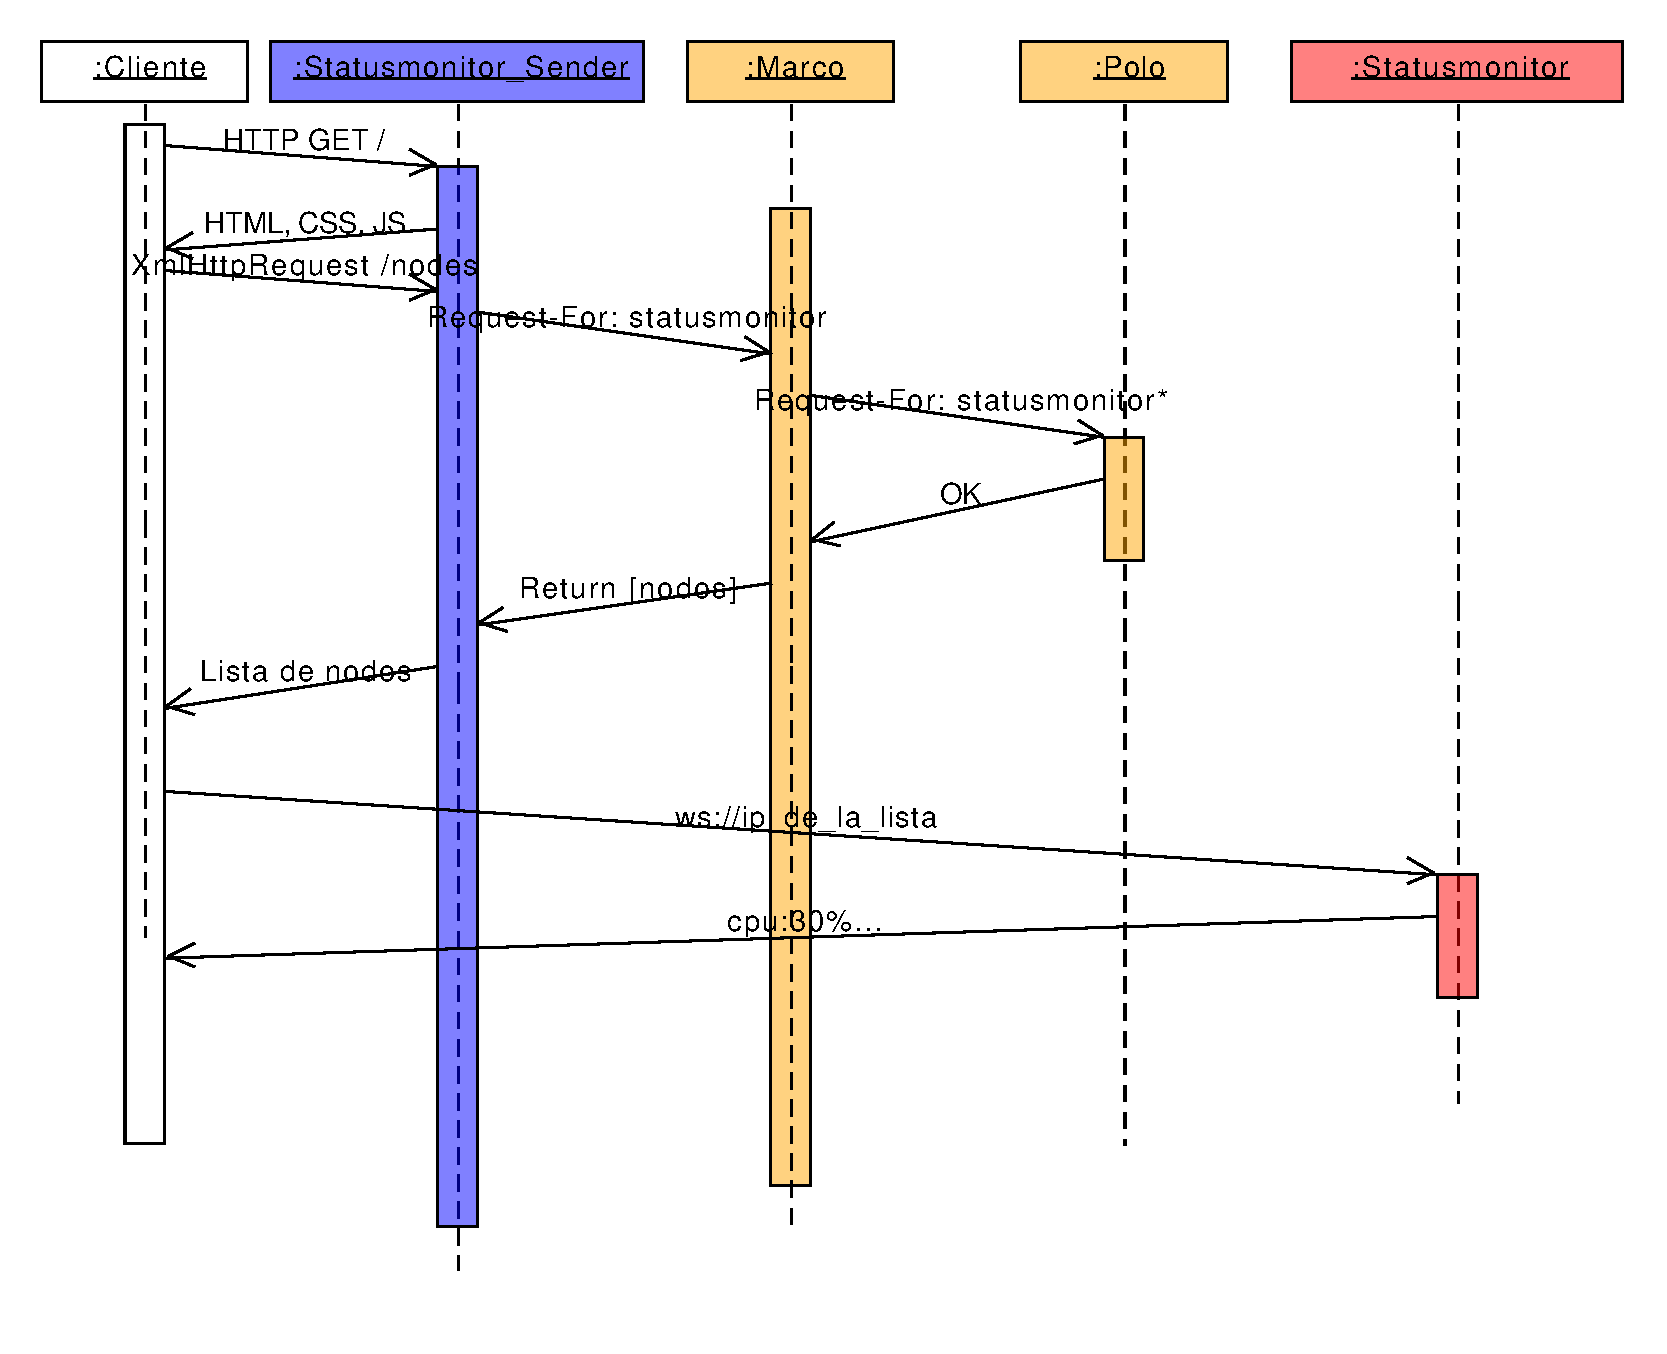
\includegraphics[width=\textwidth]{Diagrams/Sequence/statusmonitor}
% \caption[Interacción completa del usuario con \textbf{Statusmonitor}]{Interacción completa del usuario con \textbf{statusmonitor}. Los mensajes a grupos \textit{multicast} se indican con ``*''}. El usuario se conecta a la página web, que en respuesta envía un código \textit{JavaScript} (además del código HTML y CSS) que solicita la lista de nodos disponibles. Una vez recibida la petición de los nodos disponibles, el servidor solicita dicha información a través de su instancia local de \textbf{Marco} (utilizando para ello un \textit{binding}. Cuando la instancia de \textbf{Marco} termina de recoger las respuestas, retorna la información al servidor, que a su vez retorna dicha información al cliente. Al recibir dicha información, el nodo crea una conexión \textit{Websocket} con el servicio statusmonitor que se encarga de enviar por dicha conexión la información local a intervalos de tiempo definidos.)
% \label{fig:secuencia_statusmonitor}
% \end{figure}

\begin{figure}[H]
	\centering
	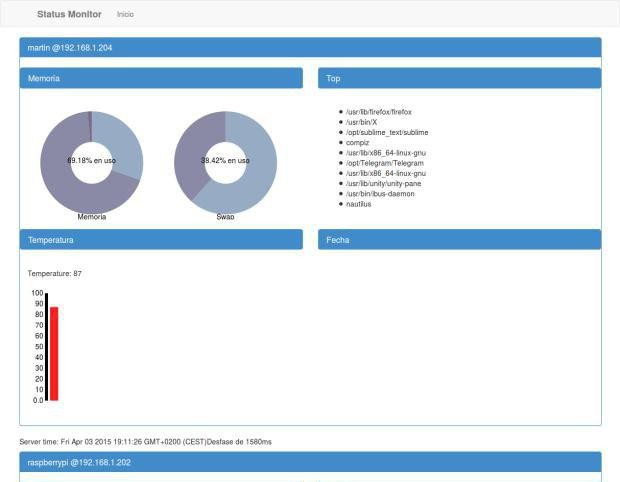
\includegraphics[width=\textwidth]{Chapter7/Figures/statusmonitor}
	\caption[Vista de la interfaz web de \textbf{Statusmonitor} una vez obtenidos los nodos]{Vista de la interfaz web una vez obtenidos los nodos y establecida la conexión a los mismos. Se observa el porcentaje de memoria y principal y de intercambio utilizadas, la temperatura del procesador, los procesos con más consumo de CPU} %TODO: y el porcentaje de CPU utilizado en cada núcleo.
	\label{fig:vista_statusmonitor}
\end{figure}

Para conocer la información sobre el sistema el proceso servidor utiliza varios comandos y ficheros auxiliares, destacando:
%TODO
\begin{itemize}
\item \texttt{top} Para conocer la información sobre los procesos más activos
\item El directorio \texttt{/proc} para conocer estadísticas del sistema como la memoria total, libre y en caché
\item El directorio \texttt{/sys} para conocer características del hardware como la temperatura
\item Comandos como \texttt{uptime} o \texttt{hostname} para conocer diversos parámetros del sistema.
\item Herramientas como \texttt{awk}, \texttt{grep} o \texttt{cut} para obtener las cadenas de interés dentro del comando de respuesta.
\end{itemize}

Dichos comandos son ejecutados periódicamente mediante el gestor de eventos \texttt{ioloop} de \textbf{Tornado}.

La implementación del servicio está realizada íntegramente en Tornado\footnote{Más información sobre el proyecto puede encontrarse en \href{http://www.tornadoweb.org/en/stable/}{tornadoweb.org/en/stable}}, un servidor web ligero asíncrono implementado íntegramente en Python y mantenido por Facebook.

\section{Deployer}

El \textbf{Deployer} es una herramienta concebida a partir de la necesidad observada entre los estudiantes de las asignaturas Sistemas Distribuidos y Arquitectura de Computadores (como se refleja en las diferentes evaluaciones realizadas, ver \ref{chapter:evaluaciones}), de replicar de una forma sencilla un ejecutable entre los diferentes nodos que conformarán el sistema distribuido.

Actualmente la infraestructura cuenta con un servidor NFS que posibilita la disponibilidad de la información en varios nodos de forma sencilla, mediante la copia a uno de los directorios alojados en el servidor. Sin embargo, este enfoque presenta varios inconvenientes: en el aspecto técnico supone una gran cantidad de ancho de banda consumido de forma continua (debido a que todos los estudiantes utilizan la misma infraestructura y realizan un gran número de operaciones de lectura y escritura a estos directorios, ralentizando el funcionamiento general del sistema enormemente) y en el aspecto didáctico, fomenta un mal hábito, pues los estudiantes no conocen otra forma de realizar despliegues más allá de la copia utilizando una interfaz gráfica y accediendo físicamente al nodo (si bien esta situación se mitiga en la asignatura Sistemas Distribuidos, donde deben automatizar los despliegues). Además, es necesario disponer de acceso físico a cada uno de los nodos, o en su defecto, conocer sus direcciones de red para realizar un acceso remoto.

Con el objetivo de proporcionar una alternativa adecuada a las necesidades y problemas descritos, surge esta herramienta, que aprovecha la funcionalidad de \textbf{MarcoPolo} para realizar su cometido.

La herramienta permite realizar las siguientes tareas de forma sencilla:

\begin{itemize}
\item Conocer todos los nodos disponibles sobre los que se podrá realizar el despliegue y seleccionar sobre cuáles de ellos trabajar.
%\item Conocer la situación de cada nodo en tiempo real, aprovechando la herramienta \textbf{statusmonitor}, cuya funcionalidad se integra en este sistema.
\item Permitir la copia a dichos nodos.
\item Posibilitar la ejecución de comandos de forma remota una vez que el despliegue ha sido realizado.
\item Facilitar la integración con contenedores de servicios, tales como \textbf{Apache Tomcat}.
\end{itemize}

La aplicación es accesible a través de un panel web %TODO: o del comando marcodeploy
. La interfaz web permite además conocer el estado de cada nodo en tiempo real, funcionalidad que a través de la línea de órdenes está disponible a través de los comandos %TODO: marcostatus

\begin{figure}[H]
\centering
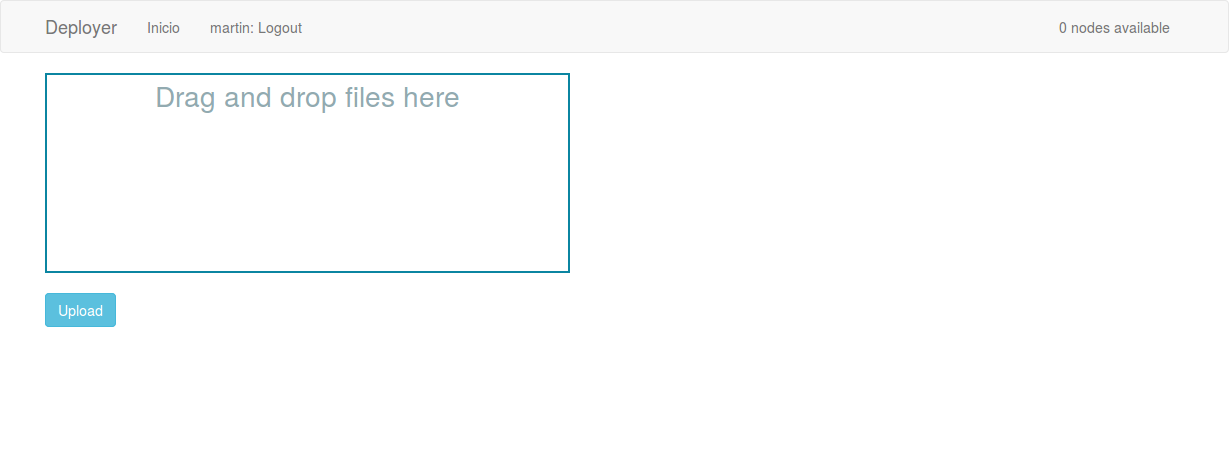
\includegraphics[width=\textwidth]{Chapter7/Figures/deployer}
\caption[Interfaz web del deployer]{Interfaz web del deployer. A la izquierda figuran los controles y a la derecha la lista de nodos sobre los que se puede realizar el despliegue}
\label{fig:vista_deployer}
\end{figure}

Al igual que en el caso de la aplicación \textbf{statusmonitor} el \textbf{deployer} está creado utilizando el servidor web \textbf{Tornado} y todo el contenido enviado al usuario se reduce a archivos HTML, CSS y JavaScript. La comunicación entre el cliente y el servidor se realiza a través de peticiones \textit{AJAX} y \textit{Websockets}. Todo el control de la interfaz se delega a hojas de estilo CSS y JavaScript utilizando la biblioteca jQuery\footnote{\href{https://jquery.com/}{jquery.com/}}.

\paragraph{Autenticación}

La autenticación de los usuarios se realiza mediante el módulo \textbf{PAM} presente en cada nodo\cite{osf:rfc86}, utilizando \textbf{python-pam} para el acceso al mismo desde \textbf{Python}\cite{python-am}.

%TODO: \begin{figure}[H]
% \centering
% %\includegraphics[width=\textwidth]{Chapter7/Sequence}
% %\caption{Diagrama de secuencia de la interacción}
% %\label{fig:sequence_deployer}
% \end{figure}

\section{Logger}

Uno de los aspectos que dificultan el desarrollo de aplicaciones distribuidas son las tareas de análisis y depuración del código desarrollado. Soluciones ``creativas'' como utilizar el puerto GPIO\footnote{\href{http://elinux.org/RPi\_Serial\_Connection}{http://elinux.org/RPi\_Serial\_Connection} Uso del puerto GPIO como conexión serie.} para este tipo de tareas son efectivas, si bien no aplicables a cualquier dispositivo o aplicación (por ejemplo, un ejecutable que no pueda ser modificado). Se debe por tanto buscar una solución complementaria para este tipo de casos.

El \textbf{logger} es una herramienta que, a través de WebSockets y redireccionamiento de \textit{streams}, permite enviar la salida que una aplicación emite a través de los canales estándares (\textbf{stdout}, \textbf{stderr}) a una interfaz web.

Esta herramienta se integra con el \textbf{deployer}, mostrando la salida por pantalla del comando ejecutado por pantalla\citationneeded[Ejecución del comando en m nodos. m < n (conjunto de los seleccionados). ¿Botón de selección?]. Una vez que se completa el despliegue, se ejecutará el comando indicado en el panel de subida.

El usuario puede además enviar señales de terminación al proceso a través de la interfaz, útiles en situaciones en las que el programa se comporta de forma errónea o incontrolada. Se enviará una señal de terminación que, en caso de no surtir efecto, será sucedida por una señal \textbf{kill}. 

La gestión de esta funcionalidad se realiza a través del bucle de eventos de \textbf{Tornado}, añadiendo al bucle de eventos de la aplicación web el descriptor de fichero de las salidas \textbf{stdout} y \textbf{stderr} del proceso que ejecuta el comando.

\subsection{Marcoshell}

Marcoshell sigue un funcionamiento similar al de \textbf{logger}. La diferencia clave es la independencia de \textbf{deployer}. La herramienta simula una consola que implementa un subconjunto de la funcionalidad esperada de una consola tradicional. Incluye también funcionalidad para el envío de señales de terminación.

\section{Herramientas de gestión}

\subsubsection{MarcoBootstrap}

Uno de los mayores problemas a la hora de gestionar un sistema con un número de componentes elevado es la instalación de todos los componentes y la actualización de los mismos. \textbf{MarcoBootstrap} es una herramienta que posibilita la instalación del sistema operativo de forma autónoma y que únicamente requiere la copia en la tarjeta SD del sistema de un pequeño conjunto de utilidades, cuyo tamaño es 33 \textit{megabytes}.

%\ref{marcobootstrap}




\subsection{Herramientas didácticas}

\subsubsection{The LED API}

\subsubsection{MusicPI}


\subsection{Pruebas de concepto}

%\includegraphics{Chapter7/ScreenShot.png}http://www.bootc.net/archives/2012/05/26/how-to-build-a-cross-compiler-for-your-raspberry-pi/
